\documentclass[UTF8, twoside]{EPURapport}
\usepackage{algpseudocode}
\usepackage{algorithm}
\usepackage{pdfpages}
\usepackage[nottoc, notlof, notlot]{tocbibind}
\usepackage{amsmath,amsfonts,amsthm}
\usepackage{graphicx}
\usepackage{rotating}
\usepackage{color}
\usepackage{colortbl}
%\usepackage{listings}

%\renewcommand{\lstlistlistingname}{Liste des codes}
%\renewcommand{\lstlistingname}{Code}

%\addextratables{%
%	\lstlistoflistings
%}

%\swapAuthorsAndSupervisors



\thedocument{Operational research project report}{Ant colony optimization algorithm for a combined routing and scheduling problem}{Ant colony optimization algorithm for a combined routing and scheduling problem}

\grade{Computer Aided Decision Support\\ International Research Master 2\\ 2013 - 2014}

\authors{%
	\category{Student}{%
		\name{Thomas NOGUER} \mail{thomas.noguer@etu.univ-tours.fr}
	}
	\details{M2RI CADS 2013 - 2014}
}

\supervisors{%
	\category{Supervisors}{%
		\name{Jean-Charles BILLAUT} \mail{jean-charles.billaut@univ-tours.fr}
		\name{Nicolas MONMARCHÉ} \mail{nicolas.monmarche@univ-tours.fr}
	}
	\details{Université François-Rabelais, Tours}
}

\abstracts{This document presents an implementation of the ant colony metaheuristic for a combined routing and scheduling problem along with another simple heuristic. The results and comparison between those two methods are part of this report.}
{Combined scheduling routing, ant colony, optimization, heuristic, metaheuristic, flowshop, batching}

\begin{document}

\chapter{Introduction}

	\hspace{4ex}An unexplored topic in scheduling is the mixed problems. This domain is vast and contains a wide variety of problems. Some mixed problems can be very close to other known problems or the problems they are composed of. However there is another sort of mixed problems that can change the way we approach the original problems completely. Our problem is from this second part, it is a combination of a flowshop, a travelling salesman and a batching problem.
	
	We can picture this problem as follows: a factory with two machines in a flowshop are producing objects that need to be delivered to different locations. The produced objects have a limited lifespan, they must reach their destination before a certain date. The objects once produced are organised in delivery batches. A unique truck is making the deliveries of the batches choosing a certain delivery route between the factory and the different destinations of the objects. We want to minimise the tardiness of arrival of the objects to their destination, we do not want the objects to reach their destination after their expiration date. The problem can be resumed in three steps:
\begin{itemize}
\item[$\bullet$] Organise the production of the objects on the two production machines of the flowshop,
\item[$\bullet$] Organise the produced objects into delivery batches,
\item[$\bullet$] Choose a delivery route for each delivery batch between the factory and the destinations.
\end{itemize}

	The travelling salesman problem is known to be NP-hard, our problem contains the travelling salesman problem we can deduce the complexity of our combined routing and scheduling problem as being NP-hard. This is for this reason that we don't try to solve the problem at the optimality, we will look for non-optimal approaches.

	In this project, we want to try a first approach of the problem with a metaheuristic: the ant colony. The ant colony can be used in order to take into account several constrains which is the case of our combined problem.
	\\
	
	The rest of this report features the formalization of the problem, the general definitions of the ant colony metaheuristic, the ant colony heuristic applied to our problem, the results of this heuristic, the perspectives the project and finally the assessment of this project in regard of my scholarship.

\chapter{Formalization of the problem}

	The problem can be defined from three different sub-problems :
	
\begin{itemize}
\item[$\bullet$] The two machines permutation flowshop. We have two machines $M_1$ and $M_2$ organized as a flowshop. A set of $n$ jobs have to be scheduled into a sequence. Each job $j$ has a value $a_j$ and $b_j$ that correspond to the time required to complete the job $j$ on $M_1$ and $M_2$ respectively.
\item[$\bullet$] The batching of jobs to be delivered. When the jobs are completed for the two machines permutation flowshop we must form batches of jobs, where a batch must contain at least one job. These groups are then used for the third sub-problem.
\item[$\bullet$] A travelling salesman problem. We consider one truck taking the groups of jobs previously formed where each job has a destination $k_j$. The idea is to find the sequence of destinations in order to deliver every job from the batch while minimizing the travelling distance. We have a matrix $K$ ($m \times m$) where $m$ is the number of destinations and $K_i^j$ is the distance between the destination $i$ and $j$. It is important to know that every delivery has to start from the factory and come back to the factory after delivering every jobs. The factory is always the destination 0 in the matrix $K$.
\end{itemize}

	The objective function is to minimize the sum of tardiness of the jobs $\overset{j \leq n}{\underset{j=1}{\sum}} T_j$. The tardiness $T_j$ of a job is defined as follows: $T_j = max(L_j, 0)$ where the lateness $L_j$  of a job $j$ is the difference between the completion time of the job $C_j$ and its due date $d_j$: $L_j = C_j - d_j$. The completion time of a job is not equal to the completion time of the job for the flowshop problem but for the travelling salesman problem. $C_j$ is equal to the date at which the truck is coming back to the factory after its deliveries.
	We consider that the truck has no capacity limit, it can carry has many jobs has possible.
\\

	The input data of our problem are the following :
\begin{itemize}
\item[$\bullet$] The number $n$ of jobs,
\item[$\bullet$] The values $a_j$, $b_j$ and $d_j$ of job $j$ ($\forall j \in [1,n]$),
\item[$\bullet$] The number of $m$ of destinations,
\item[$\bullet$] The destination $k_j$ of job $j$ ($\forall j \in [1,n]$),
\item[$\bullet$] The matrix $K$ ($m \times m$) of distances between each destination.\\
\end{itemize}

	During the resolution of the problem we must find the sequence of jobs on the flowshop, the groups of jobs to be delivered and the sequence of delivery for each group.

	We proposed a first way of encoding a solution : a table of size $n$ containing the sequence of job for the flowshop sub-problem, a table of size $2n$ containing the groups and sequences for the travelling salesman sub-problem. The first cell of the second table contains the number of jobs for the first group, the following cells contain the id of jobs in the delivery sequence and so on. The figure \ref{problem} shows a solution for a simple instance of the problem with its encoding. 
	
	The sequence here is $\{1,2,3\}$ the first batch $G_1$ of jobs is $G_1 = \{1,2\}$ and 1 is delivered first, the second batch $G_2$ only contains one job $G_2 = \{3\}$.
	
	
\begin{figure}
	\centering 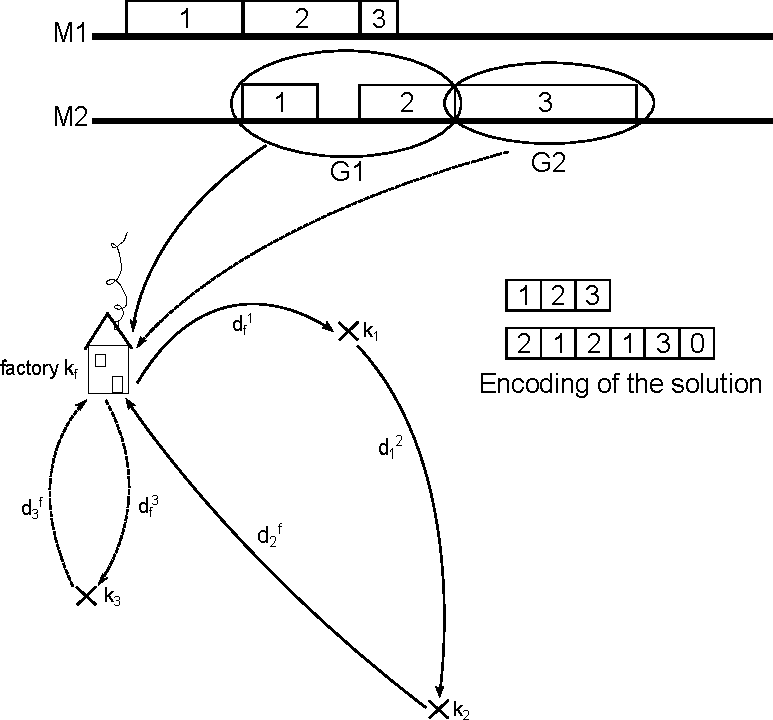
\includegraphics{images/problem.pdf}
	\caption {A solution of the problem for a simple instance}	
	\label {problem}
\end{figure}

\chapter{Ant colony optimization}

\section{General definitions}

 	\hspace{4ex}In this part, we will consider a travelling salesman problem in order to explain the mechanism of the ant colony metaheuristic. The graph representation of cities is an intuitive approach for such a method.
	
	
	The classic algorithm of an ant colony heuristic is the following :

\begin{algorithm}
  \caption{Ant colony}
  \begin{algorithmic}[1]
      \For{$k \gets 1 \textrm{ to } iterationsNumber$}
      	\For {\textbf{each} $ant$}
        	\State Construct solution
			\State Local pheromone update
        \EndFor
        \State Local search
        \State Global pheromone update
      \EndFor
      \State \textbf{return} Best found solution
  \end{algorithmic}
\end{algorithm}

	In order to construct the solution we need a probability formula based on the following :
	\\

\[
P^m_{ij}= \left\{ 
\begin{array}{l r}
\frac{[\tau_{ij}]^\alpha \cdot [\eta_{ij}]^\beta}{\underset{l\notin tabu_m}{\sum}[\tau_{il}]^\alpha \cdot [\eta_{il}]^\beta} & \text{if } j\notin tabu_m\\
0 & \text{if } j\in tabu_m
\end{array}
\right.
\]

	Where $P^m_{ij}$ is the probability of an ant $m$ in city $i$ to go to the city $j$, $\tau{ij}$ the intensity of the pheromone trail from $i$ to $j$, $\eta_{ij}$  the visibility of city $j$ from city $i$ (this is typically $1/d_{ij}$ where $d_{ij}$ is the distance between $i$ and $j$). $\alpha$ and $\beta$ are parameters used to make the pheromone trail or the visibility more important from one another. And finally, the tabu list is used to prevent ants from going to forbidden cities like the city they come from.
\\

	The local pheromone update is used to emulate the evaporation phenomenon of pheromone. This evaporation is calculated from a formula based on the following :
	\\
	
\[
\tau_{ij} = (1-\rho) \cdot \tau_{ij}+\rho \cdot \tau_{0}
\]

	Where $\rho$ is the evaporation rate and $\tau_{0}$ the minimum value of the pheromone trail, which is also usually used as initial value. It is important to consider that the evaporation function is only used for the paths the ants travelled through.
\\

	The global pheromone update is used to emulate the deposit of pheromone from the ants. Again this function is only used for the edges the ant travelled while forming its solution. This deposit is calculated from a formula based on the following :
	\\
	
\[
\tau_{ij} = (1-\rho) \cdot \tau_{ij}+\rho \cdot \Delta\tau_{ij}
\]

	Where $\Delta\tau_{ij}$ is the improvement rate between the new best solution and the previous best solution.

\section{Application to the combined routing and scheduling problem}

\label{Ant colony heuristic}

	\hspace{4ex}One main issue to overcome here is the fact that there is no simple graph representation of the complete problem. For the travelling salesman problem, it is easy to see how the pheromone trails and the visibilities come from. For our problem it is quite different. We can try to imagine a graph that an ant could visit and form a complete solution from it. For instance, a node could represent the fact that a job $j$ is placed first in the flowshop, alone in a delivery group and delivered first. But we then have to consider every possibility knowing that the grouping and delivering problems are dependant on the flowshop. If we change the sequence of jobs in the flowshop we obtain a different grouping problem and then a different travelling salesman problem.
	
	Even though we happen to be able to model such graph, its size would be unreasonably huge. It is not rational to chose such solution. We must abandon the idea to apply the ant colony optimization all at once for our problem and think of a different approach.
	\\
	
	Instead of trying to use the ant colony metaheuristic for the complete problem, we can consider using it for parts of it. We can chose to use the ant colony on one or several sub-problem and use different method to construct the rest of the solution and then update the pheromone trails based on the results of the whole solution.
	
	Although is not clever to consider using the ant colony for the travelling salesman sub-problem since the problem is different each time you change the groups to be delivered or the sequence of jobs from the flowshop. The pheromone trails would be lost each time you change the solution in any sub-problem above.
	
	We can still consider the other two sub-problems as potential candidate for the ant colony. Indeed, the flowshop problem and the grouping problem can both be considered central in our global problem. We then have three possibilities, use the ant colony on the flowshop, on the grouping problem or both and use simple heuristics coupled with a surrogate mechanism to obtain the value of the objective function for our solution in order to guide the ants towards the best solution. The surrogate mechanism could be very useful in order to save time computation, it would be used in the majority of cases and replaced with heuristics in the others in order to verify if the current solution is still a good one.
\\	

\subsection{Definition of the Ant colony for the mixed optimisation problem}
	
	\hspace{4ex}Here we decided to use the ant colony metaheuristic on the batching problem. It is easy to find heuristics to construct the rest of the solution when we have the groups of jobs. We have to specify how to implement the ant colony algorithm to our sub-problem. This typical visualisation we use for an ant building a solution is the complete graph of cities of the travelling salesman problem. The nodes of the graph are cities, when the ant goes from city $a$ to city $b$ is means we have the sequence $ab$ in our solution. The ant has to visit all nodes with a specific path. It chooses a path from the probability formula defined before.
	
	We use a different construction of solution for our algorithm. We take the jobs as the nodes of the graph and two edges (a green and a red) connecting each node together. The graph has then $n$ nodes and $n(n+1)$ edges. During the construction of a solution, and ant can come from a node $a$ to a node $b$ from two different edges: If it takes the green edge, it means node $a$ and $b$ belong to the same batch. If it takes the red edge, it means the two nodes do not belong to the same batch. The figure \ref{ant_colony_graph} shows how to construct the batches from the path travelled by an ant on our graph.
\\

\begin{figure} [h]
	\centering 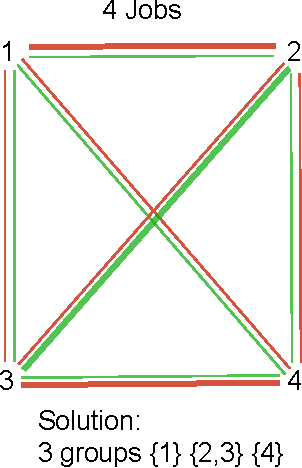
\includegraphics{images/ant_colony_graph.pdf}
	\caption {The construction of a solution by an ant.}	
	\label {ant_colony_graph}
\end{figure}

	We know how the ants construct the solution and how the graph is made. We need to define the visibility criterion for each edge of our graph. Let's define the visibility for the green edges, what is the formula that will make the ants form groups of jobs? We are handling a complex problem, we need to take into account the two other sub-problems: the flowshop, and the travelling salesman.
\\
	
	For the travelling salesman what we wish to do is group the jobs if their distance is small: $\frac{1}{\delta_{ij}}$ where $\delta_{ij}$ is the distance between the destination of job $i$ and the destination of job $j$. 
	
	For the deliveries we know that we have to start from the factory and to end at the factory, the distance between the destinations of the jobs and the factory matters, when the jobs are far from the factory we tend to form groups: $\frac{\delta_{0i} \cdot \delta_{0j}}{\delta_{max}}$ where $\delta_{0i}$ is the distance between the factory and the destination of job $i$ and $\delta_{max}$ is the maximum distance between the factory and any other destination. We divide by the maximum value in order to keep a value between 0 and 1.
	
	We can then combine those two criteria and add a tuning parameter $\omega$ to make one criterion or the other more important: 
\\

\[
\left(\frac{1}{\delta_{ij}}\right)^\omega \cdot \frac{\sqrt{\delta_{0i} \cdot \delta_{0j}}}{\delta_{max}}
\]
\\

	With this criterion, we will form batches of jobs the further their destinations are from the factory and the closer their destinations are from one another.
\\

	For the flowshop sub-problem we want to consider the due dates of the jobs. When the due dates of two jobs are close to each other we will tend to put them into the same group: 
\\

\[
\frac{1}{\vert d_i - d_j \vert}
\]
\\

	We can combine the criterion from both sub-problem, add tuning parameters and get the formula of the visibility $\eta_{ij}$:
\\

\[
\eta_{ij}^g = 
\left( \frac{1}{\vert d_i - d_j \vert} \right)^\psi \cdot \left[\left(\frac{1}{\delta_{ij}}\right)^\omega \cdot \frac{\sqrt{\delta_{0i} \cdot \delta_{0j}}}{\delta_{max}} \right]^\chi \text{, if } \vert d_i - d_j \vert = 0 \text{ then } \frac{1}{\vert d_i - d_j \vert} = 1 \text{ and if } \delta_{ij} = 0 \text{ then } \frac{1}{\delta_{ij}} = 1
\]
\\

	We said before that this visibility was to be considered for the green edges of our graph. The visibility $\eta_{ij}^{r}$ for the red edges is the complement criteria of the visibility of the green edges:
\\

\[
\eta_{ij}^{r} = 1 - \eta_{ij}^g
\]
\\
	
	One last point needs to be defined: How do we choose the edges during the construction of a solution? When forming the batches, an ant has to choose an edge from the node it currently stands to another node. We have our probability formula defined before:
	
\[
P^m_{ij}= \left\{ 
\begin{array}{l r}
\frac{[\tau_{ij}]^\alpha \cdot [\eta_{ij}]^\beta}{\underset{l\notin tabu_m}{\sum}[\tau_{il}]^\alpha \cdot [\eta_{il}]^\beta} & \text{if } j\notin tabu_m\\
0 & \text{if } j\in tabu_m
\end{array}
\right.
\]
	
	To make its choice an ant follows the following algorithm:
	
\begin{algorithm}
	\caption{Choosing an edge going from node $i$}
	\begin{algorithmic}[1]
		\State $a \gets $ Random number $\in \left[0;1\right]$ 
		\If {$a > P_0$}
			\State \Return Edge with highest $P^m_{ij}$
		\Else
			\State $b \gets $ Random number $\in \left[0; \underset{j}{\sum}\tau_{ij}\right]$
			\State $t \gets 0$
			\State $k \gets 1$
			\While {$t < b$}
				\State $t \gets t + \tau_{ik}$
				\State $k \gets k + 1$
			\EndWhile
			\State \Return Edge $k$
		\EndIf
	\end{algorithmic}
	\label{roulette}
\end{algorithm}

	This value $P_0$ is a diversification probability, it is typically equal to 0.2. It means that 80\% of the time the ant will take the edge with the maximum value of $P^m_{ij}$, and 20\% of the time the ant will choose a random edge using the sum of $\tau_{ij}$ as probability repartition. The point of such a mechanism is to allow the ants to choose edges disregard their visibility and with a random value in order to diversify the solutions and be able to explore new paths.

\subsection{Algorithms}

	Let us call our search graph $G$, the node set of this graph $\mathscr{N}$, the green edge set $\mathscr{G}$ and the red edge set $\mathscr{R}$. 

\begin{algorithm}
  \caption{Ant colony for the mixed optimisation problem}
  \begin{algorithmic}[1]
  	  \State Initialize pheromone matrix with $\tau_0$
  	  \State Calculate the matrix of visibility
  	  \State List $path$
      \For{$k \gets 1 \textrm{ to } iterationsNumber$}
      	\For {\textbf{each} $ant$}
      		\State \textit{/* Construction of the solution for the grouping problem*/}
			\State Select random node $u$ from $\mathscr{N}$
    		\State $i \gets 1$
    		\Repeat
    			\State Select an edge $v$ going from $u$ with algorithm \ref{roulette}
   				\State $path.push(v)$
   				\State $u \gets $ node connected to $v$
   				\State $i \gets i+1$
    		\Until $i = n$
    		\State Each community of nodes linked with edged from $path$ form a group
    		\State Each remaining nodes form an individual group containing only this node
    		\State \textit{/* Construction of the rest of the solution */}
    		\State Use heuristics to construct the rest of the solution
    		\State Computation of $\underset{i}{\sum} T_i$
    		\If{the new solution is better than the best known solution}
    			\State Save the new solution as the new best known solution
    		\EndIf
			\State Local pheromone update
        \EndFor
        \State Local search
        \State Global pheromone update (see algorithm \ref{global_update})
      \EndFor
      \State \textbf{return} Best found solution
  \end{algorithmic}
\end{algorithm}

\begin{algorithm}
	\caption{Global pheromone update}
	\begin{algorithmic}[1]
		\State $\%improvement \gets (oldBestSolution - newBestSolution) / newBestSolution$
		\State $path \gets newBestSolution.getPath()$
		\For {\textbf{each} edge $e$ in $path$}
			\If {$edge.color = green$}
				\State // $\tau_0$ is the minimal pheromone value, $\tau_{ij}^g$ is the pheromone on the green edge between $i$ and $j$ and $\rho$ is the evaporation rate.
				\State $i \gets edge.start$ 
				\State $j \gets edge.end$
				\State $\tau_{ij}^g = (1-\rho) \cdot \tau_{ij}^g + \rho \cdot \%improvement$
				\State $\tau_{ji}^g = \tau_{ij}^g$
			\Else
				\State $\tau_{ij}^r = (1-\rho) \cdot \tau_{ij}^r + \rho \cdot \%improvement$
				\State $\tau_{ji}^r = \tau_{ij}^r$
			\EndIf
		\EndFor
	\end{algorithmic}
	\label{global_update}  	  
\end{algorithm}

\clearpage

	When we have formed the batches of jobs, we have to deduce the rest of the solution. In order to do so, we use simple heuristics. To form the sequence of the flowshop problem, we order the batches in increasing order of the minimum due date of the jobs within the batch. The jobs of a batch are then scheduled following Johnson's algorithm.
	
	The final part to form our solution is to find the delivery order of the jobs of a batch. To do so, we use the nearest neighbour criterion. For each jobs of a batch, take the nearest neighbour until all the jobs of the batch are processed. We apply this rule to each batch to obtain the fully formed solution.
\\

	The method explained above is the first one ever tried on this problem. In order to be able to evaluate its performance we need another one to serve as comparison. It is in that purpose that we proposed a simple heuristic to solve the problem. The heuristic is actually formed of three methods, one for each sub-problem:
\begin{itemize}
\item[$\bullet$] Johnson's algorithm is used to find the sequence of jobs for the flowshop,
\item[$\bullet$] The batches are formed with a simple method. We follow the sequence of jobs formed by the algorithm and decide to put a job into the current batch or to create a new one if the choice gives gives a lesser $\sum T$ than the other.
\item[$\bullet$] For each batch we choose the delivery order of the jobs following the nearest neighbour criterion.
\end{itemize}

	This simple heuristic is used to see if a naive approach is more efficient that our less naive once.
	
\chapter{Results}

	\hspace{4ex}This part presents the results obtained during this project. The value $v$ correspond to the idle time of the truck, the truck is idle when it is not delivering. The value $w$ correspond to the idle time of the jobs, a job is idle when it is completed on the flowshop and waits to be delivered.
	
	Also each row of $n$ resumes 10 instances. The following simple generation has been used to create the instances:
\begin{itemize}
\item[$\bullet$] 10 instances per value of $n$,
\item[$\bullet$] $n \in \{10; 20; 50\}$,
\item[$\bullet$] $m = n+1$,
\item[$\bullet$] $a_i \in \left[1,100\right]$, $\forall i \in [0, n]$
\item[$\bullet$] $b_i \in \left[1,100\right]$, $\forall i \in [0, n]$
\item[$\bullet$] $d_i \in \left[(\gamma-\alpha)\cdot100, (\gamma+\alpha)\cdot100)\right]$, $\forall i \in [0, n]$
\item[$\bullet$] $k_i \in \left[1,m\right]$, $\forall i \in [0, n]$
\item[$\bullet$] $K_{ij} = $ Manhattan($x_i,y_i,x_j,y_j$), $\forall i,j \in [0,m]$
\item[$\bullet$] $x_i \in \left[0,50\right]$, $\forall i \in [0,m]$
\item[$\bullet$] $y_i \in \left[0,50\right]$, $\forall i \in [0,m]$
\item[$\bullet$] $\alpha = 0.5$,
\item[$\bullet$] $\gamma = 0.5$.\\
\end{itemize}

	The used parameters for the ant colony are the following: 
\begin{itemize}
\item[$\bullet$] Number of iterations $= 50$,
\item[$\bullet$] Number of ants $= 10$,
\item[$\bullet$] $P_0 = 0.2$,
\item[$\bullet$] $\tau_{0} = 0.1$,
\item[$\bullet$] $\rho = 0.1$,
\item[$\bullet$] $\alpha = \beta = \psi = \omega = \chi = 1$.
\end{itemize}

\begin{table}[!h]
\centering
\tabcolsep=0.11cm
\setlength{\extrarowheight}{1.5pt}
\begin{tabular}{|c|c|c|c|c|c|c|c|c|c|c|c|c|} 
\hline
 & \multicolumn{12}{c|}{Heuristics} \\
\hline
n & $\sum T_{min}$ & $\sum T_{avg}$ & $\sum T_{max}$ & \begin{sideways} Time(s)$_{min}$ \end{sideways} & \begin{sideways} Time(s)$_{avg}$ \end{sideways} & \begin{sideways} Time(s)$_{max}$ \end{sideways} & $\% v_{min}$ & $\% v_{avg}$ & $\% v_{max}$ & $\% w_{min}$ & $\% w_{avg}$ & $\% w_{max}$\\
\hline
10 & 2735 & 3483.3 & 4327 & 0 & 0 & 0 & 3 & 22 & 40 & 2 & 15 & 26\\
\hline
20 & 11995 & 13345.1 & 14885 & 0 & 0 & 0 & 0 & 11 & 24 & 19 & 61 & 95\\
\hline
50 & 71125 & 82427.7 & 89546 & 0 & 0 & 0 & 3 & 12 & 25 & 50 & 70 & 90\\
\hline
\textbf{AVG} & \textbf{28618.33} & \textbf{33085.37} & \textbf{36252.67} & \textbf{0} & \textbf{0} & \textbf{0} & \textbf{2}  & \textbf{15} & \textbf{30} & \textbf{24} & \textbf{49} & \textbf{70}\\
\hline
\end{tabular}
\caption{\label{tab:Heuristics}Results for heuristics}
\end{table}

\begin{table}[!h]
\centering
\tabcolsep=0.11cm
\setlength{\extrarowheight}{1.5pt}
\begin{tabular}{|c|c|c|c|c|c|c|c|c|c|c|c|c|} 
\hline
 & \multicolumn{12}{c|}{Ants} \\
\hline
n & $\sum T_{min}$ & $\sum T_{avg}$ & $\sum T_{max}$ & \begin{sideways} Time(s)$_{min}$ \end{sideways} & \begin{sideways} Time(s)$_{avg}$ \end{sideways} & \begin{sideways} Time(s)$_{max}$ \end{sideways} & $\% v_{min}$ & $\% v_{avg}$ & $\% v_{max}$ & $\% w_{min}$ & $\% w_{avg}$ & $\% w_{max}$\\
\hline
10 & 2899 & 32767.90 & 5177 & 0.01 & 0.01 & 0.01 & 30 & 42 & 57 & 0 & 8 & 18\\
\hline
20 & 13528 & 14043.20 & 14766 & 0.02 & 0.02 & 0.02 & 27 & 41 & 59 & 0 & 9 & 26\\
\hline
50 & 72856 & 82069.80 & 87965 & 0.07 & 0.08 & 0.09 & 42 & 52 & 59 & 0 & 9 & 25\\
\hline
\textbf{AVG}& \textbf{29761} & \textbf{33293.63} & \textbf{35969.33} & \textbf{0.03} & \textbf{0.03} & \textbf{0.04} & \textbf{33} & \textbf{45} & \textbf{58} & \textbf{0} & \textbf{9} & \textbf{23}\\
\hline
\end{tabular}
\caption{\label{tab:ants}Results for the ant colony}
\end{table}

\begin{table}[!h]
\centering
\setlength{\extrarowheight}{1.5pt}
\begin{tabular}{|c|c|c|c|c|c|c|} 
\hline
 & \multicolumn{6}{c|}{Ants - Heuristics} \\
\hline
n & $\Delta \sum T_{min}$ & $\Delta \sum T_{avg}$ & $\Delta \sum T_{max}$ & \begin{sideways}$\Delta$ Time(s)$_{min}$ \end{sideways} & \begin{sideways}$\Delta$ Time(s)$_{avg}$ \end{sideways} & \begin{sideways}$\Delta$ Time(s)$_{max}$ \end{sideways}\\
\hline
10 & \cellcolor{red}164 & \cellcolor{red}284.6 & \cellcolor{red}850 & \cellcolor{red}0.01 & \cellcolor{red}0.01 & \cellcolor{red}0.01\\
\hline
20 & \cellcolor{red}1533.00 & \cellcolor{red}698.10 & \cellcolor{green}-119 & \cellcolor{red}0.02 & \cellcolor{red}0.02 & \cellcolor{red}0.02\\
\hline
50 & \cellcolor{red}1731 & \cellcolor{green}-357.9 & \cellcolor{green}-1581 & \cellcolor{red}0.07 & \cellcolor{red}0.08 & \cellcolor{red}0.09\\
\hline
\textbf{AVG} & \cellcolor{red}\textbf{1142.667} & \cellcolor{red}\textbf{208.27} & \cellcolor{green}\textbf{-283.33} & \cellcolor{red}\textbf{0.03} & \cellcolor{red}\textbf{0.03} & \cellcolor{red}\textbf{0.04}\\
\hline
\end{tabular}
\caption{\label{tab:diff}Difference of the results between the ant colony and the heuristics}
\end{table}

\clearpage

	A couple of things are to be noticed from those result tables. Firstly, in average the ant colony heuristic gives worst results in exception of the instances of 50 jobs. The execution time of the ant colony is higher which was to be expected but still insignificant. One last interesting datum is the $\%v_{avg}$ and $\%w_{avg}$ for both the ant colony and the heuristics: the ant colony tends to have the truck wait, when for the heuristics it is the jobs. One concern at the beginning of this project was to be able to generate instances that are not too easy on the flowshop part or too easy on the travelling salesman part. This is why we showed the values $v$ and $w$ to be able to evaluate this criterion. It occurs here that both methods have a different tendency, we can think that our instances are good enough.


\chapter{Perspectives}

	\hspace{4ex}This project is the first on such problem, there is still much to do and to explore. One first thing to do is to change the values of the parameters of the ant colony and see how they influence the results. It should be possible to enhance the current results in this way. The second thing is to implement a local search for both the ant colony and the heuristic to see how it can affect the results. The study of the instances and the behaviour of the solution couple with the values of $v$ and $w$ on each method could help understand the mechanisms of the problem and how to improve our methods.
	
	Also there is always to possibility to find different resolution methods for this problem and different instance generations.

\chapter{Assessment}

	\hspace{4ex}This project was very enriching, the problem is completely unexplored and it was very interesting to see how we can use the ant colony for this problem. It was also the first time I used the ant colony metaheuristic in a project and helped me grasp the machinery behind it.
\\

	This project was not easy and I had some difficulties along it. The first difficulty was the application of the ant colony metaheuristic to our problem as explained at the beginning of the part \ref{Ant colony heuristic}. Also the project required a lot of implementation in a short amount of time. I did my best to make the code clear and commented so it could be reused for future projects.

\chapter{Conclusion}

	\hspace{4ex}I hope that my work will be useful for future work on this problem, and will help to provide good results to show at the ROADEF conference of 2014. I would like to conclude by thanking both supervisors of this project Jean-Charles Billaut and Nicolas Monmarché for their time, help and sympathy.

\begin{thebibliography}{99}

\bibitem{GG10}
{\sc Marc Gravel, Caroline Gagné}
{\ "Ant colony optimization for manufacturing aluminum bars."}.
{ \textit{Chapter 7} from the book \textbf{Artificial Ants} \textit{From collective intelligence to real-life optimization and beyond}, Nicolas Monmarché, Frédéric Guinand, Patrick Siarry 2010}.

\end{thebibliography}

\end{document}
